\begin{enunciado}{\ejercicio}
  Sea $v \en \complejos^n$ un vector columna tal que $\norma{v}_2 = 1$. Probar que:
  \begin{enumerate}[label=(\alph*)]
    \item La transformación lineal definida por la matriz $vv^*$ es la proyección ortogonal sobre $\ket{v}$.

    \item Si $\set{v_1,\ldots,v_m}$ es una base ortonormal del subespacio $S$, entonces
          $A = \sumatoria{i=1}{m}v_iv_i^*$ es la proyección ortogonal sobre $S$.

    \item Si $A$ es como en el ítem anterior, $I-A$ es la proyección ortogonal sobre $S^\perp$.

    \item Eligiendo $v \en \reales^2$ tal que $\norma{v}_2 = 1$, corroborar gráficamente en \python que $R = I - 2vv^*$
          es la reflexión respecto de $\ket{v}^\perp$.
  \end{enumerate}
\end{enunciado}

\begin{enumerate}[label=(\alph*)]
  \item\label{ej-17:itema} Tenemos que:
        $$
          \norma{v}_2 = 1
          \Sii{def}
          v^* \cdot v \igual{$\llamada1$} 1
        $$
        Un \textit{proyector ortogonal sobre $\ket{v},\, P$ cumple}:
        $$
          P \cdot v \igual{def} v
          , \quad
          P \cdot v^\perp \igual{def} 0
          , \quad
          P = P^*
          \quad \ytext \quad
          \nucleo{P}
          \perp
          \imagen{P}
        $$
        Entonces si esta \textit{gaver} $vv^*$ cumple eso, ganamos {\tiny\poo}:
        $$
          \ob{vv^*}{P} \cdot v \igual{\red{!}}
          v (v^* \cdot v) \igual{$\llamada1$} v,
        $$
        \textit{that was easy}. Vamos a por la otra. Agarro algún $w \en \complejos^n$:
        $$
          \begin{array}{rcl}
            vv^* \cdot \ub{(Pw - w)}{\perp v} = 0
             & \sii           &
            vv^* \cdot Pw - vv^* \cdot w = 0 \\
             & \Sii{\red{!}}  &
            v(P^*v)^* w - vv^*  w = 0        \\
             & \Sii{\red{!!}} &
            v(Pv)^* w - vv^*  w = 0          \\
             & \Sii{def}      &
            vv^* w - vv^*  w \igual{\checkmark} 0
          \end{array}
        $$
        Me doy cuenta que podría haber probado que $(vv^*)^* = vv^*$ ¿Pero quien me quita lo bailado?:

  \item Si tengo una base del subespacio, entonces puedo escribir a un vector genérico $w \en S$ como una combineta de
        los vectores de la base:
        $$
          w = \sumatoria{\blue{j} = 1}{m} a_{\blue{j}} v_{\blue{j}} = a_1 v_1 + a_2  v_2 + \cdots + a_n v_n
        $$
        Transformo teniendo en cuenta que
        $
          v_{\red{i}}^* (a_{\blue{j}} v_{\blue{j}}) =
          \llave{rcl}{
            a_{\red{i}} & \text{ si } & \red{i} = \blue{j}\\
            0 & \text{ si } & \red{i} \distinto \blue{j}
          }
        $, recordando que $\norma{v_i}_2 = 1$:
        $$
          Aw = \sumatoria{\red{i}=1}{m}v_{\red{i}}v_{\red{i}}^* w = \sumatoria{\red{i} = 1}{m} a_{\red{i}}v_i = w
          \entonces Aw = w
        $$
        Me doy cuenta que podría haber probado que $A = A^*$ ¿Pero quien me quita lo bailado?:
        $$
          A^* =
          \left(\sumatoria{\red{i}=1}{m}v_{\red{i}}v_{\red{i}}^*\right)^*
          \igual{\red{!}}
          \sumatoria{\red{i}=1}{m}\left(v_{\red{i}}v_{\red{i}}^*\right)^* =
          \sumatoria{\red{i}=1}{m}v_{\red{i}}v_{\red{i}}^* = A
        $$

  \item Medio que usé algo de esto en el ítem \ref{ej-17:itema}. Un \textit{proyector ortogonal} sobre $S$, va
        a mandar todo elemento del \textit{complemento ortogonal} de $S,\, S^\perp$ al 0.

        Es decir, si $w \en S^\perp$:
        $$
          A w = 0
          \quad \ytext \quad
          (I - A)w = w
          \entonces
          A \ub{(I - A)w}{w} =
          (A - A^2)w
          \igual{\red{!}}
          (A - A )w = 0.
        $$
        Podemos decir que $A(I - A)$ es el operador nulo.
        
        En general para cualquier elemento $\green{v}$ del \textit{espacio vectorial} $V$: Puedo escribir $v = s + s^\perp$,
        una combineta única de elementos de $S \ytext S^\perp$, ya que $S \sumaDirecta S^\perp$.
        $$
          A(I - A) v = A(I - A)(s + s^\perp) = A(s + s^\perp - As - As^\perp) = As + As^\perp - As - A^2s^\perp \igual{\red{!}} 0
        $$
        Los \textit{proyectores ortogonales} cumplen que $\nucleo(P) \perp \imagen(P)$, donde la imagen es el $S$ al que se proyecta y
        el núcleo es el $S^\perp$.

  \item Sí,lo sé, esto no es una implementación en \python.

        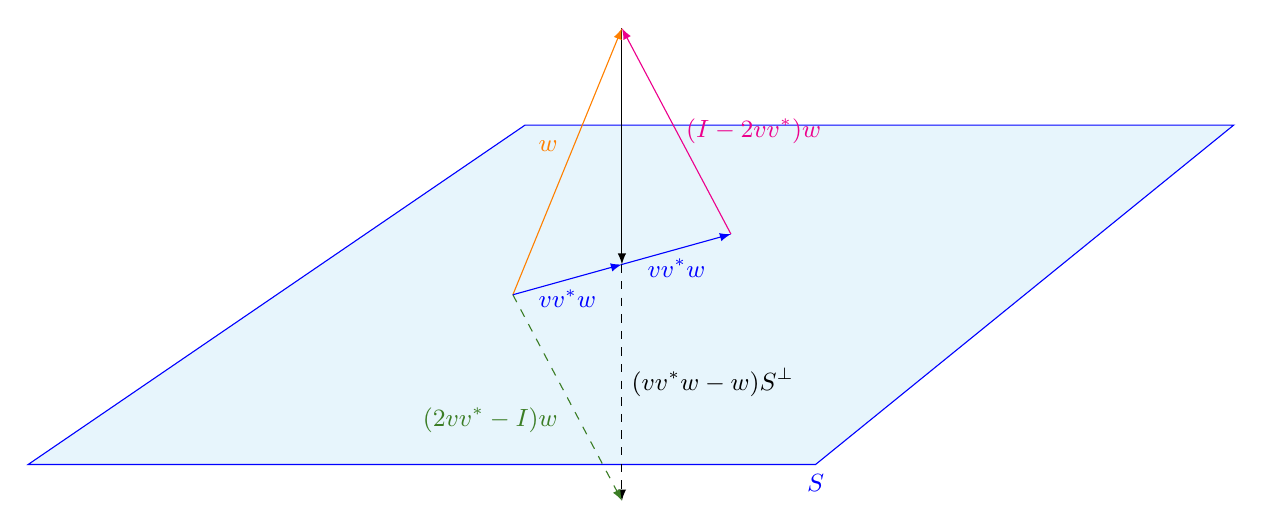
\begin{tikzpicture}[baseline=0, every node/.style={font=\small}]
          \coordinate[] (A) at (0,1,0);
          \coordinate[] (B) at (-4,-1,6);
          \coordinate[] (C) at (6,-1,6);
          \coordinate[] (D) at (9,1,0);
          \coordinate[] (P) at (2,3,2);
          \coordinate[] (Q) at (1,0,3);
          \coordinate[] (PP) at (2,0,2);
          \coordinate[] (Pref) at (3,0,1);
          \coordinate[] (Psim) at (2,-3,2);
          \draw[blue, fill=Cerulean!10] (A)--(B)--(C) node[below] {$S$}--(D)--cycle;
          \draw[thin,-latex, black,dashed] (PP)--(Psim) node[midway,right]{$(vv^*w - w) \en S^\perp$} ;
          \draw[thin,-latex, black] (P)--(PP) node[midway,right]{} ;
          \draw[-latex,orange] (Q)--(P) node[midway,above left]{$w$};
          \draw[-latex, magenta] (Pref)--(P) node[midway,right]{$(I - 2vv^*)w$};
          \draw[-latex,OliveGreen, dashed] (Q)--(Psim) node[midway,below left]{$(2vv^* - I)w$};
          \draw[blue,-latex] (Q)--(PP) node[midway, below]{$vv^*w$};
          \draw[blue,-latex] (PP)--(Pref) node[midway, below]{$vv^*w$};
        \end{tikzpicture}

\end{enumerate}

\begin{aportes}
  \item \aporte{\dirRepo}{naD GarRaz \github}
\end{aportes}
